% Created 2025-05-15 Thu 22:00
% Intended LaTeX compiler: pdflatex
\documentclass[11pt]{article}
\usepackage[utf8]{inputenc}
\usepackage[T1]{fontenc}
\usepackage{graphicx}
\usepackage{longtable}
\usepackage{wrapfig}
\usepackage{rotating}
\usepackage[normalem]{ulem}
\usepackage{amsmath}
\usepackage{amssymb}
\usepackage{capt-of}
\usepackage{hyperref}
\usepackage{mathptmx}  % Times font
\usepackage{helvet}   % Helvetica font
\renewcommand{\familydefault}{\sfdefault} % Sans-serif as default
\usepackage{titlesec}
\usepackage{lmodern}
\usepackage{tikz}
\author{Serob Tigranyan}
\date{\today}
\title{Matematiks}
\hypersetup{
 pdfauthor={Serob Tigranyan},
 pdftitle={Matematiks},
 pdfkeywords={},
 pdfsubject={},
 pdfcreator={Emacs 30.1 (Org mode 9.7.26)}, 
 pdflang={English}}
\begin{document}

\maketitle
\tableofcontents

\newpage
\section{Analysis of the Function}
\label{sec:orge65d9a3}
Given the function:
\[
f(x)=\frac{x^2+3x-1}{3-2x}
\]

Analyze it and graph the function by following the steps below:
\begin{enumerate}
\item Finding the Doamin of the Function
\item Limits at the Boundaries of the Domain
\item Interceptions with Coordinate Axies
\item Critical Points and Monotonic Intervals
\item Local Extrema and values at Extrema
\item Inflection Points and Concavity
\item Identification of Asymptotes Using Limits
\item Function graph
\end{enumerate}
\section{Finding the Domain of the Function}
\label{sec:orga637b0a}
We'll first need to find the domain of the function as this step is essential when observing the function at bounderies which it is undefined.
Because our function is rational, the domain of the function would be the following:
\[
3-2x \neq 0 \rightarrow x \neq \frac{3}{2}
\]

Therefore the domain of \(f(x)\) is:
\[
\left(-\infty, \frac{3}{2} \right) \cup \left( \frac{3}{2}, +\infty \right)
\]

\newpage
\section{Limits at the Boundaries of the Domain}
\label{sec:org04da1c5}
We examine the behaviour near the point where the function is undefined (\(x=\frac{3}{2}\)) from both sides.

As \(x \to \frac{3}{2}^+\):
\[
\lim_{x \to -\infty} \frac{x^2+3x-1}{3-2x} = \lim_{x \to -\infty} \frac{x \left( x + \frac{3}{x} - \frac{1}{x^2} \right)}{ x \left( \frac{3}{x} - 2 \right) } = \frac{-\infty}{-2} = +\infty
\]

As \(x \to \frac{3}{2}^-\):
\[
\lim_{x \to +\infty} \frac{x^2+3x-1}{3-2x} = \frac{ \infty }{-2} = -\infty
\]

\[
\lim_{x\to\frac{3}{2}^+} \frac{x^2+3x-1}{3-2x} = \lim_{x\to\frac{3}{2}^+} x^2+3x+1 \lim_{x\to\frac{3}{2}^+} \frac{1}{3-2x} = \frac{31}{4} \cdot \frac{1}{3-3} = +\infty
\]

\[
\lim_{x\to\frac{3}{2}^-} \frac{x^2+3x-1}{3-2x} = = -\infty
\]
\section{Interceptions with Coordinate Axies}
\label{sec:orgaa58ef3}
We find where the function intercepts at \(x\) and \(y\) axies by plugging zero for each axies.

X Interception:
\[
x^2+3x-1=0
\]

Using the quadratic formula we get:
\[
x = \frac{-3 \pm \sqrt{13}}{2}
\]

Y Interception:
\[
(0)^2+3(0)-1 = -1
\]

\newpage
\section{Critical Points and Monotonic Intervals}
\label{sec:org9e1f265}
Critical points occur in a function where the derivative is zero. To find the critical points we first differentiate the function and then solve for zero.

Differentiate:
\[
f'(x) = \frac{d}{dx} \left( \frac{x^2+3x-1}{3-2x} \right) = \frac{-2x^2+6x+7}{(3-2x)^2}
\]

Solve for zero:
\[
\frac{-2x^2+6x+7}{(3-2x)^2} = 0 \rightarrow 2x^2-6x-7=0 \rightarrow x_1 = \frac{6 \pm \sqrt{94}}{4} \rightarrow x_2 = \frac{3 \pm \sqrt{23}}{2}
\]

We have two critical points:
\[
x_1 = \frac{3 + \sqrt{23}}{2}
\]
\[
x_2 = \frac{3 - \sqrt{23}}{2}
\]
\section{Local Extrema and values at Extrema}
\label{sec:org12b56a9}
To find the monotonic intervals we first compute the derivate then find the signs on the interval.
\subsection{Monotonic Intervals}
\label{sec:orgc149bdb}
Monotonicity:
\[
f'(x) > 0 \ \ increasing 
\]
\[
f'(x) < 0 \ \ decreasing
\]

Pick something lesser than \(x_1\), bigger than \(x_1\) and finally bigger than \(x_3\) and also plug in the values that are undefined as well:
\newpage
\[
f'(-1) = -0.04 \ \ decreasing 
\]
\[
f'(\frac{3}{2}) = 1.5 \ \ increasing
\]
\[
f'(2) = 11 \ \ increasing
\]
\[
f'(4) = -0.04 \ \ decreasing
\]

Therefore our monotonic intervals are:
\[
Increasing: \left( \frac{3-\sqrt{23}}{2} ; \frac{3+\sqrt{23}}{2} \right)
\]
\[
Decreasing: \left( -\infty ; \frac{3 - \sqrt{23}}{2} \right) \cup \left( \frac{3 + \sqrt{23}}{2} ; \infty \right)
\]
\subsection{Local Extrema}
\label{sec:org415f045}
To find the local extrema of the function we take the interval from before and determine whether the function at the critical point is a minimum or a maximum.
\begin{center}
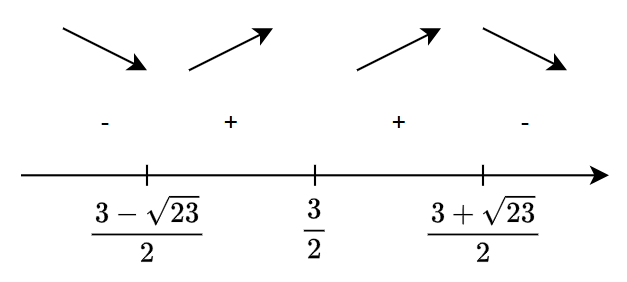
\includegraphics[width=.9\linewidth]{./skarmbild.png}
\end{center}

If the function is decreasing before critical point \(x\) and increasing afterwards then its a local minimum, otherwise its a local maximum.

Therefore:
\[
x_{min} = \frac{3-\sqrt{23}}{2}
\]
\[
x_{max} = \frac{3+\sqrt{23}}{2}
\]
\subsection{Evaluation of Function Values at Local Extrema}
\label{sec:org0530f9b}
We simply plug in the extrema values into the function to get their values:
\[
f(\frac{3-\sqrt{23}}{2}) = \frac{1}{2} \left( \sqrt{23} - 6 \right)
\]
\[
f(\frac{3+\sqrt{23}}{2}) = -3-\frac{\sqrt{23}}{2}
\]
\section{Inflection Points and Concavity}
\label{sec:org9c19472}
To find the Inflection Points and Concavity, we'll first need to find the second derivative of the function:
\[
f'(x) = \frac{-2x^2+6x+7}{(3-2x)^2}
\]
\[
f''(x) = \frac{d}{dx} \left( \frac{-2x^2+6x+7}{(3-2x)^2} \right) = \frac{\left( -2x^2+6x+7 \right)' \left( 3-2x \right)^2 - \left( -2x^2+6x+7 \right) \left(\left( 3 - 2x\right)^2\right)'}{\left(3-2x\right)^4}
\]
\[
f''(x) = \frac{46}{(3-2x)^3}
\]

Afterwards in our Interval we plug in Critical Values inside the second derivative from which we can tell the following:
\begin{itemize}
\item \(f''(x) > 0\): Concave up
\item \(f''(x) < 0\): Concave down
\end{itemize}

After plugging our Critical Values we get:
\[
f''\left(\frac{3+\sqrt{23}}{2}\right) \approx -0.41
\]
\[
f''\left(\frac{3-\sqrt{23}}{2}\right) \approx 0.41
\]

\newpage
Therefore:
\begin{center}
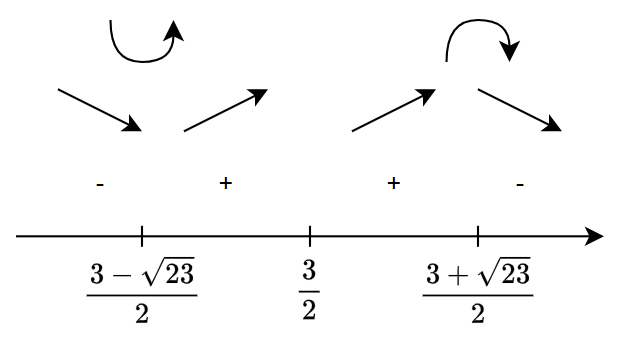
\includegraphics[width=0.3\textwidth]{./skarmbild2.png}
\end{center}

To find the Inflection Points we zero the second derivative and solve:
\[
\frac{46}{(3-2x)^3} = 0
\]

But as we can see this equation has no Real solution therefore another possible candidate is \(\frac{3}{2}\) but our function here is undefined therefore \textbf{our function has no Inflection Points.}
\section{Identification of Asymptotes using Limits}
\label{sec:orgff4b913}
\subsection{Vertical Asympotote}
\label{sec:org757784c}
Vertical asymptotes occur near unbounded \(x\) values for \(f(x)\), to find whether or not an unbounded \(x\) for the function is an asymptote, we simply take the limit from both sides of \(x\).

\(x\) from right:
\[
\lim_{x\to\frac{3}{2}^+} \frac{x^2+3x-1}{3-2x} = +\infty
\]

\(x\) from left:
\[
\lim_{x\to\frac{3}{2}^-} \frac{x^2+3x-1}{3-2x} = -\infty
\]
\subsection{Slant Asymptote and Horizontal Asymptote}
\label{sec:orge886423}
Slant Asymptotes occur when finding \(k\), \(b\) and plugging them in the linear equation below:
\[
y=kx+b
\]

We determine whether or not we have a Slant or Horizontal Asymptotes by looking at each coefficient:
\begin{itemize}
\item \(k\) and \(b\) are both constants: We have a Slant Asymptote
\item \(b\) is a constant and \(k\) is zero: We have a Horizontal Asymptote
\end{itemize}

Now we find \(k\) by taking the limit as \(x \rightarrow \pm \infty\):
\[
k=\lim_{x\to\pm\infty} \frac{f(x)}{x} \rightarrow \lim_{x\to\pm\infty} \frac{x^2+3x-1}{x(3-2x)} = \frac{1+0-0}{0-2} = \frac{1}{-2}
\]

Now we find \(b\) by plugging in \(k\) and taking the limit as \(x \rightarrow \pm \infty\):
\[
b=\lim_{x\to\pm\infty} f(x)-kx \rightarrow \lim_{x\to\pm\infty} \left( \frac{x^2+3x-1}{3-2x} + \frac{x}{2} \right) = \frac{9-0}{0-4} = -\frac{9}{4}
\]

And finally we get the linear function below:
\[
y=kx+b \rightarrow y=\frac{x}{-2}-\frac{9}{4}
\]

As we can see, neither \(k\) or \(b\) are zero therefore we have a Slant Asymptote.
\section{Function graph}
\label{sec:org5b3a6f4}
\begin{center}
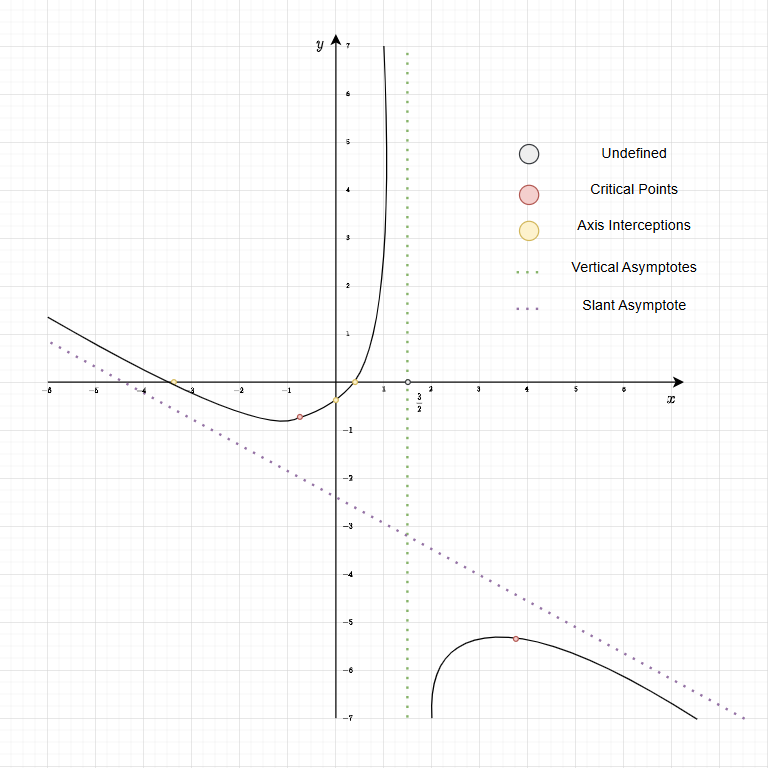
\includegraphics[width=.9\linewidth]{./holy_balony.png}
\end{center}
\end{document}
